\chapter{\IfLanguageName{dutch}{Stand van zaken}{State of the art}}%
\label{ch:stand-van-zaken}

% Tip: Begin elk hoofdstuk met een paragraaf inleiding die beschrijft hoe
% dit hoofdstuk past binnen het geheel van de bachelorproef. Geef in het
% bijzonder aan wat de link is met het vorige en volgende hoofdstuk.

% Pas na deze inleidende paragraaf komt de eerste sectiehoofding.

Het genereren van kunstwerken op basis van tekstuele input heeft de afgelopen jaren aanzienlijke vooruitgang geboekt dankzij de opkomst van generatieve AI-technieken. Deze technieken maken gebruik van geavanceerde deep learning-algoritmen om kunstwerken te creëren die uniek zijn en vaak verrassend creatief. In deze literatuurstudie zullen we ons richten op de generatieve benadering van het creëren van kunstwerken, waarbij we dieper ingaan op de methoden en technieken die worden gebruikt om deze werken te genereren. \\

We zullen een uitgebreid overzicht geven van de huidige stand van zaken op het gebied van generatieve kunst, met specifieke nadruk op het gebruik van tekstuele input als basis voor het genereren van kunstwerken. We bespreken de evolutie van traditionele machinale vertaling en samenvatting naar de meer geavanceerde generatieve algoritmen die tegenwoordig worden toegepast. Door middel van deze algoritmen worden tekstinvoer omgezet in beelden, schilderijen, muziekstukken en andere vormen van kunst. \\

Binnen het domein van generatieve kunst zullen we specifiek kijken naar het gebruik van webscraping als een methode om tekstuele input te verzamelen voor het genereren van kunstwerken. We zullen de werking van deze methode bespreken, inclusief de uitdagingen die kunnen optreden bij het verkrijgen en verwerken van tekstuele gegevens van het web. Bovendien zullen we onderzoeken hoe webscraping kan worden toegepast om informatie te verzamelen die als input kan dienen voor het genereren van unieke en expressieve kunstwerken. \\

Al met al zal deze literatuurstudie een diepgaand inzicht bieden in de generatieve benadering van het creëren van kunstwerken op basis van tekstuele input. We zullen de huidige stand van de technologie onderzoeken, de potentie ervan in verschillende toepassingsgebieden bespreken en nadenken over mogelijke toekomstige ontwikkelingen op dit boeiende gebied.
\pagebreak


\section{Generatieve AI}

Generatieve AI is een subdomein van kunstmatige intelligentie dat zich richt op het creëren van nieuwe, unieke content op basis van bestaande gegevens. Het maakt gebruik van geavanceerde technieken zoals deep learning om patronen en relaties in de data te identificeren en te leren. Dit stelt de AI in staat om innovatieve en creatieve oplossingen te genereren voor verschillende toepassingen, zoals het genereren van kunstwerken op basis van tekstuele input \autocite{SonixAI2021}\\

Een voorbeeld van een toepassing van generatieve AI is het RobotReporter-project, uitgevoerd aan de Hogeschool Utrecht. Dit project onderzoekt de mogelijkheden van generatieve AI-systemen om journalistiek werk te automatiseren. Het project richt zich op het gebruik van webscraping en natural language processing (NLP) om informatie te verzamelen en te verwerken, en vervolgens met behulp van generatieve AI-algoritmen nieuwe content te creëren \autocite{HU2021}. Dit kan leiden tot efficiëntere en snellere nieuwsproductie. \\

Binnen de paper geschreven door Microsoft en OpenAI beschrijven ze de impact van generatieve AI op de arbeidsmarkt. Daarin wordt beschreven dat hoe langer en zwaardere studies je doet en dus hoe hoger het gemiddelde loon is binnen uw functie, hoe meer taken generatieve AI kan doen in plaats van de actor zelf. \autocite{gpt_micai} \\ 

Generatieve AI heeft niet alleen invloed op de hogerbetaalde jobs, maar ook op andere beroepen. Een artikel van Harvard Business Review bespreekt de impact van generatieve AI op klantenserviceberoepen \autocite{HBR2023}. In plaats van banen te vervangen, wordt betoogd dat generatieve AI klantenservicemedewerkers kan ondersteunen en hun werk kan verbeteren. Door geautomatiseerde systemen te gebruiken om routineuze taken te voltooien, kunnen medewerkers zich concentreren op meer complexe en empathische aspecten van hun werk. \\

In de afgelopen jaren is generatieve AI een veelbelovend onderzoeksgebied geworden, met tal van toepassingen en mogelijkheden. Desondanks zijn er nog steeds uitdagingen en beperkingen die moeten worden aangepakt, zoals de  aspecten en de benodigde rekenkracht. Toekomstig onderzoek en ontwikkeling zullen waarschijnlijk leiden tot nieuwe doorbraken en toepassingen op het gebied van generatieve AI. \\

\subsection{Transformer}
Stel je voor dat je een groep vrienden hebt die allemaal tegelijkertijd praten. Je kunt aandacht besteden aan iedereen, maar afhankelijk van het onderwerp, zul je misschien meer aandacht besteden aan wat sommigen zeggen dan aan anderen. Dit is hoe transformers werken. \\

Transformers zijn een soort computermodel dat wordt gebruikt om taal te begrijpen en te genereren. In plaats van elk woord in een zin een voor een te verwerken, zoals een mens die leest, kunnen transformers naar alle woorden in een zin tegelijk kijken. Dit stelt hen in staat om de relaties tussen woorden beter te begrijpen, ongeacht hoe ver ze in de zin van elkaar verwijderd zijn. \\

Laten we een voorbeeld nemen: "Het glas brak omdat het gevallen was." Voor ons is het duidelijk dat "het" verwijst naar "het glas". Maar voor een computermodel dat woorden een voor een verwerkt, kan het moeilijk zijn om deze verbinding te maken, vooral als de zin langer is. Transformers lossen dit probleem op met iets dat we "attention" noemen. Dit betekent dat het model beslist welke delen van de zin het belangrijkst zijn om de betekenis te begrijpen, net zoals jij zou besluiten naar wie je moet luisteren in een groep vrienden.\\ 

Dit mechanisme van "attention" is niet alleen cruciaal voor het begrijpen van tekst, maar ook voor het genereren ervan, zoals in het geval van GPT. \\

GPT,, is in feite een groot transformer-model dat is getraind op een aanzienlijke hoeveelheid tekst van het internet. Tijdens deze training heeft het model een verscheidenheid aan gesprekken en schrijfstijlen 'gehoord', en met behulp van de transformer-architectuur, heeft het de onderlinge relaties tussen woorden in deze teksten leren begrijpen. \\

\subsection{GPT}
Generative Pre-trained Transformer (GPT) is een reeks taalmodellen ontwikkeld door OpenAI. Deze modellen zijn ontworpen om menselijke taal te begrijpen en te genereren met een hoge mate van nauwkeurigheid en coherentie. De reeks GPT-modellen omvat GPT-3, GPT-3.5 en GPT-4. GPT-modellen zijn relevant voor de vraag of AI in staat is kunstwerken te genereren die niet van echt te onderscheiden zijn, vanwege hun prestaties op het gebied van natuurlijke taalverwerking en tekstgeneratie. \\

In de volgende subsecties zullen we de kenmerken en prestaties van elk model bespreken, evenals hun bijdragen aan het veld van kunstmatige intelligentie en hun potentieel om kunstwerken te helpen genereren. \\

\subsubsection{GPT-3}
GPT-3, is een transformer-gebaseerd taalmodel met 175 miljard parameters. Het model heeft interessante prestaties geleverd op het gebied van natuurlijke taalverwerking en kan tekst genereren. \autocite{nytimes_gpt3}. GPT-3 kan worden gebruikt om teksten te genereren, zoals nieuwsartikelen, verhalen, gedichten en zelfs code. Hoewel het model niet perfect is en soms onjuiste of irrelevante informatie kan genereren, heeft het de aandacht getrokken van onderzoekers, technologiebedrijven en het grote publiek vanwege de veelzijdigheid en de kwaliteit van de gegenereerde tekst \autocite{wiki_gpt3}. \\

GPT-3 is gelanceerd door OpenAI en heeft een ongekende groei doorgemaakt, met een recordaantal gebruikers in korte tijd. Binnen slechts twee maanden na lancering bereikte het platform 100 miljoen gebruikers, waarmee het één van de snelst groeiende platform ooit is \ref{fig:gpt_growth}. \autocite{reuters_chatgpt}. Deze snelle groei en brede acceptatie zijn indicatief voor de potentie en relevantie van GPT-3 voor deze paper.\\

\begin{center}
    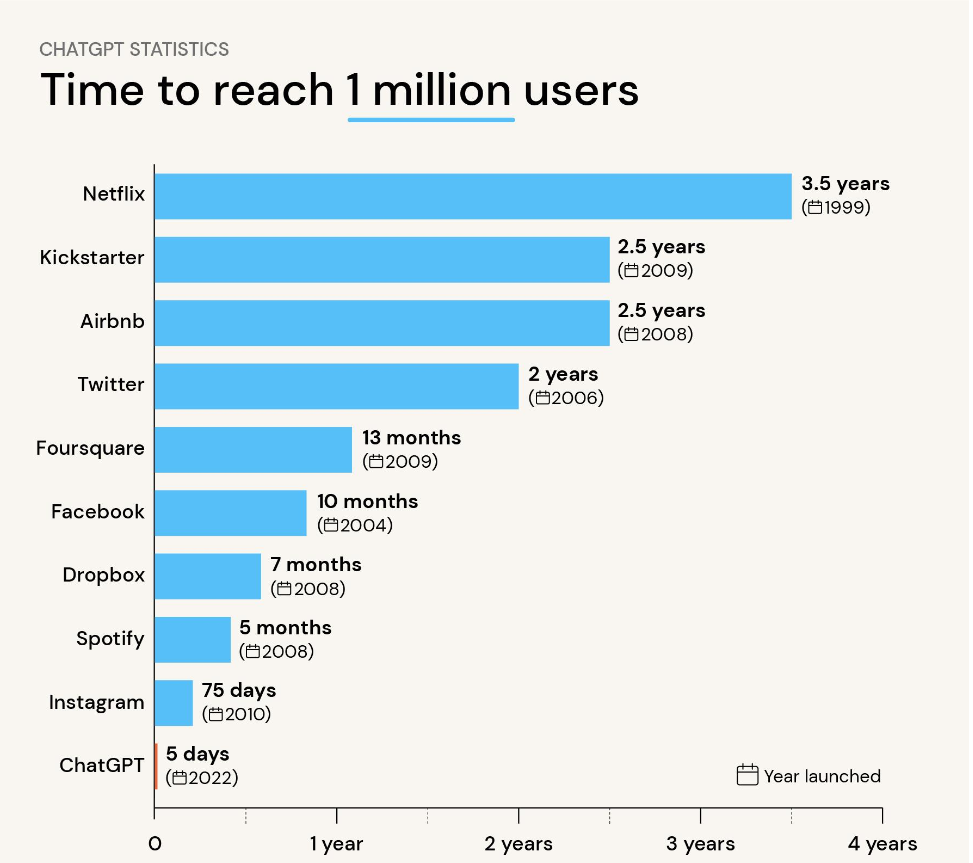
\includegraphics[width = 4in]{gpt_growth.png}
    \captionof{figure}{Tijd nodig tot 1 milioen gebruikers. \autocite{gpt_millie}}
    \label{fig:gpt_growth}
\end{center}

GPT-3 heeft een API die gebruikt kan worden.

\subsubsection{GPT-3.5}
GPT-3.5, een geüpgradede versie van het GPT-3-model, biedt geavanceerdere taalbegrip- en generatiecapaciteiten in vergelijking met zijn voorganger. De verbeteringen in GPT-3.5 stellen het model in staat om een breder scala aan complexe taken uit te voeren en betere resultaten te leveren in verschillende toepassingsgebieden, zoals tekstclassificatie, sentimentanalyse, tekstgeneratie en contextueel begrip \autocite{gpt_nappier, gpt_cn}. \\

\autocite{gpt_nappier} bespreken de technische aspecten van GPT-3.5 en de belangrijkste verschillen tussen GPT-3 en GPT-3.5. Een van de opmerkelijke verbeteringen in GPT-3.5 is het vermogen om context beter te begrijpen en relevante tekst te genereren op basis van die context. Dit is vooral belangrijk in taken waarbij contextuele informatie cruciaal is voor het begrijpen en genereren van geschikte antwoorden of voortzettingen van een tekst. \\

Een ander belangrijk aspect van GPT-3.5 is de verbeterde efficiëntie en prestaties. GPT-3.5 maakt gebruik van geoptimaliseerde architecturen en trainingsmethoden om de modelgrootte en computatievereisten te verminderen zonder concessies te doen aan de prestaties. Dit maakt het model toegankelijker en bruikbaarder voor een breder scala aan toepassingen en apparaten \autocite{gpt_nappier}. \\

\autocite{gpt_cn} verkennen de toepassingsmogelijkheden van GPT-3.5 en presenteren verschillende casestudy's die de prestaties en effectiviteit van het model aantonen. Ze onderzoeken het gebruik van GPT-3.5 in diverse domeinen, zoals het genereren van nieuwsartikelen, samenvatten van teksten, het beantwoorden van vragen op basis van tekst en het genereren van code. \\

Ondanks de goede prestaties van GPT-3.5, zijn er nog steeds uitdagingen en beperkingen die moeten worden aangepakt. In \autocite{gpt_cn} worden enkele van deze problemen besproken, zoals het genereren van irrelevante of onjuiste informatie (hallucineren), gevoeligheid voor vooroordelen in de trainingsdata en het vermogen om lange teksten te genereren zonder af te dwalen van het onderwerp. Toekomstig onderzoek zou zich kunnen richten op het verbeteren van deze aspecten en het ontwikkelen van methoden om de modelprestaties verder te verfijnen.\\

GPT-3.5 heeft een API die gebruikt kan worden onder de naam gpt-3.5-turbo. 

\subsubsection{GPT4}
GPT-4, de opvolger van GPT-3.5, is een nog geavanceerder transformer-gebaseerd taalmodel dat verder bouwt op de successen en verbeteringen van zijn voorgangers. GPT-4 biedt aanzienlijke verbeteringen op het gebied van natuurlijke taalverwerking, tekstgeneratie en begrip, evenals efficiëntie en bruikbaarheid \autocite{gpt_openai, gpt_micai}. \\

Een belangrijk kenmerk van GPT-4 is het vermogen om nog nauwkeuriger en coherenter menselijke taal te genereren en te begrijpen. Hierdoor kan GPT-4 beter presteren in verschillende toepassingsgebieden, zoals tekstclassificatie, sentimentanalyse, tekstgeneratie, contextueel begrip en vele anderen \autocite{gpt_micai}. \\

\autocite{gpt_cn} onderzoeken de technische aspecten en verbeteringen van GPT-4 ten opzichte van GPT-3.5. Ze benadrukken de geoptimaliseerde architecturen en trainingsmethoden die in GPT-4 zijn geïmplementeerd, waardoor het model betere prestaties kan leveren zonder dat dit ten koste gaat van de efficiëntie. Deze verbeteringen maken GPT-4 toegankelijker en bruikbaarder voor een breder scala aan toepassingen en apparaten. \\

Binnen het onderzoek van Microsoft \autocite{gpt_micai} toont men aan dat GPT-4 vormen van algemene intelligentie vertoont. Dit blijkt uit de kerncapaciteiten, zoals redeneren, creativiteit en deductie, expertise op verschillende onderwerpen, en de verscheidenheid aan taken die het kan uitvoeren. Hoewel er nog veel werk te doen is om een volledige AGI (Artificial General Intelligence) te creëren, wordt benadrukt dat het definiëren van intelligentie, AI en AGI complex en controversieel is en dat er geen definitieve definitie bestaat. Het onderzoek suggereert dat toekomstig werk op het gebied van GPT-4 en vergelijkbare systemen zich kan richten op het verkennen van nieuwe toepassingen en domeinen en het begrijpen van de mechanismen en principes die aan hun intelligentie ten grondslag liggen. \\

Naast de prestaties van GPT-4 hebben Elon Musk en andere experts opgeroepen tot een tijdelijke stop van Large Language Models (LLM) zoals GPT-4 kunnen overtreffen, vanwege potentiële risico's en onvoorziene gevolgen die dergelijke geavanceerde systemen met zich mee kunnen brengen zonder \autocite{reuters_musk}. 
 
\section{AI-gegenereerde kunst: tools en voorbeelden}
\subsection{ Midjourney}
Midjourney is een organisatie die met behulp van discord kunstwerken kan genereren, zo kun je een prompt sturen in de chat en krijg je verschillende kunstwerken te zien op basis van je prompt, indien je tevreden bent met de resultaten kun je de foto in hoge resultatie downloaden. Indien niet, kun je de beste van de X-aantal resultaten selecteren en hierop nieuwe resultaten laten genereren. 

\begin{center}
    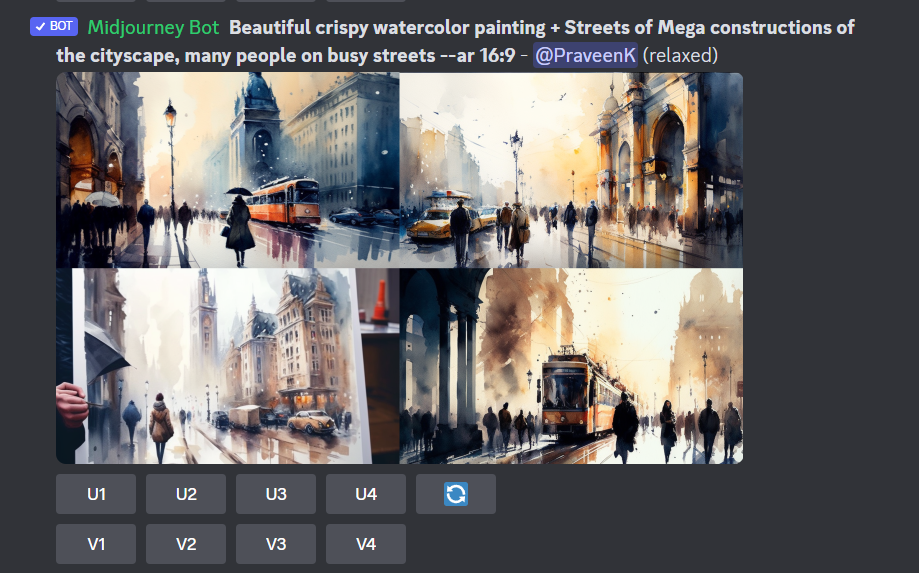
\includegraphics[width = 4in]{midjourney_ex.png}
    \captionof{figure}{Voorbeelden van AI-gegenereerde kunstwerken met behulp van Midjourney.}
    \label{fig:midjourney_ex.png}
\end{center}

Midjourney heeft geen API die we kunnen gebruiken.

\subsection{ Dall-E}
Dall-E kan gebruikt worden op de website om kunstwerkente generen maar met extra functionaliteiten vergeleken met midjourney. Dall-E laat het toe om foto's te editen en varianties van een kunstwerk te vragen. Met editen kun je een plaats markeren op het gegenereerde resultaat en hierop een nieuwe promp laten genereren, op deze manier kun je bepaalde dingen aanpassen of nieuwe attributen laten genereren op het kunstwerk. \\

Hieronder vindt u het resultaat gegenereerd op de prompt: ``Painted by Dali: Taiwan targeted by China'.' \\

\begin{figure}[h!]
    \centering
    \begin{tabular}{llll}
        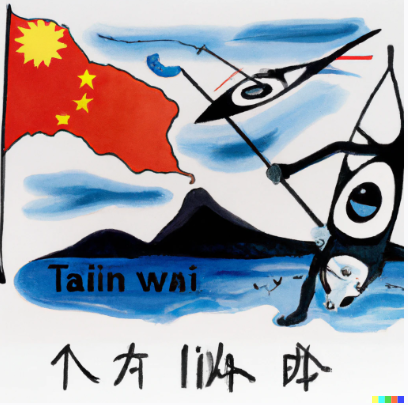
\includegraphics[width = 1.5in]{dall-e_ex1.png} &
        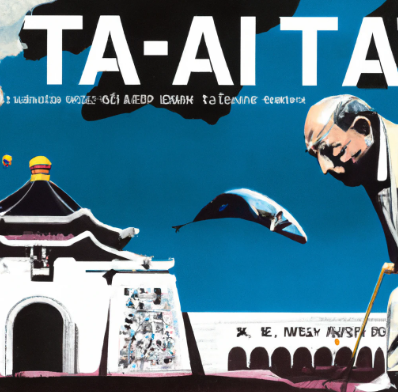
\includegraphics[width = 1.5in]{dall-e_ex2.png} \\
        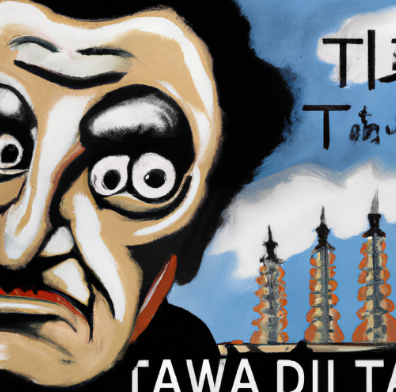
\includegraphics[width = 1.5in]{dall-e_ex3.png} &
        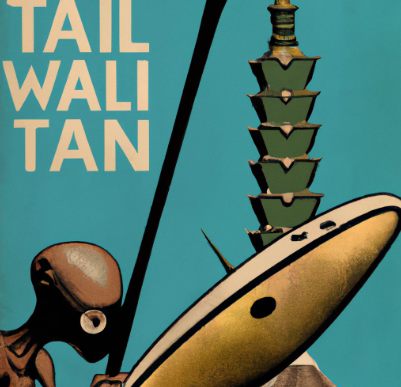
\includegraphics[width = 1.5in]{dall-e_ex4.png}
    \end{tabular}
    \caption{Voorbeelden van AI-gegenereerde kunstwerken met behulp van Dall-E.}
    \label{fig:examples}
\end{figure}


 Bovenstaande functionaliteiten worden ook aangeboden binnen de API van OpenAI.
\pagebreak

\subsection{Stable Diffusion}
Met Stable Diffusion kun je 1-4 kunstwerken laten genereren. \\

Hieronder vind u het resultaat gegenereerd op de prompt:  ``Painted by Van Gogh: War in Russia, food crisis in Asia.''

\begin{figure}[h!]
    \centering
    \begin{tabular}{llll}
        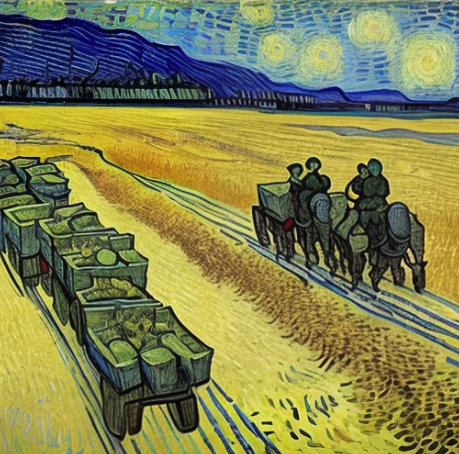
\includegraphics[width = 1.5in]{sd_ex1.png} &
        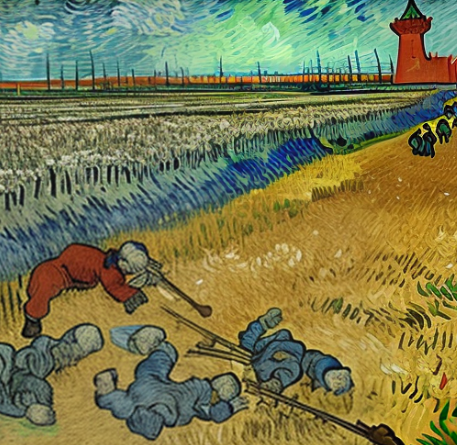
\includegraphics[width = 1.5in]{sd_ex2.png} \\
        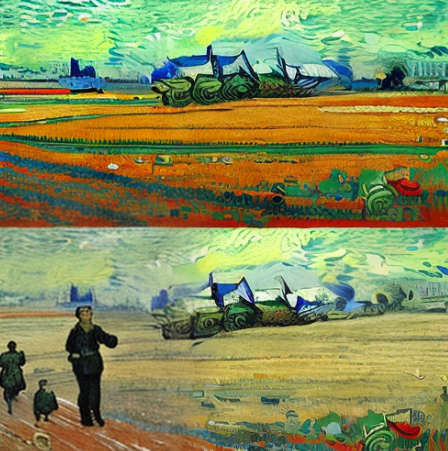
\includegraphics[width = 1.5in]{sd_ex3.png} &
        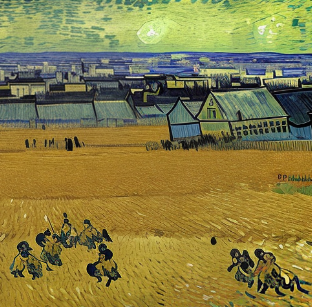
\includegraphics[width = 1.5in]{sd_ex4.png}
    \end{tabular}
    \caption{Voorbeelden van AI-gegenereerde kunstwerken met behulp van Stable Diffusion.}
    \label{fig:examples}
\end{figure}

Stable Diffusion heeft een API waarvan gebruik van gemaakt kan worden. \\

\pagebreak

\subsection{Toepassingen}
Binnen deze subsectie bespreek ik enkele toepassingen die gebruik maken van de eerder vermelde tools in punt 2.1/2.2 en 2.3.

\subsubsection{NFT's}
Een non-fungible token, beter bekend als een NFT, is een uniek digitaal object op een blockchain, meestal verbonden met speciale digitale content zoals foto's of muziek. Ze hebben een gigantische markt opgebouwd, waar individuele NFT's een waarde van miljoenen dollars kunnen bereiken \autocite{nft_whatisit}. \\

LLM's hebben het potentieel om de markt te verstoren op een manier die het menselijke aspect van NFT's kan wegnemen. In plaats van kunstenaars en creatievelingen die unieke digitale content maken, kunnen we een toekomst zien waarin AI de 'creator' wordt, wat de menselijke inspanning, creativiteit en originaliteit die traditioneel geassocieerd worden met kunst kan ondermijnen. 

\subsubsection{Graphic Design}
Binnen het domein van graphic design kunnen AI-tools zoals DALL-E en StyleGAN worden ingezet voor verschillende toepassingen. Zo kunnen ze bijvoorbeeld worden gebruikt om nieuwe verpakkingen, zoals cornflakesdozen, te ontwerpen door unieke en aantrekkelijke ontwerpen te genereren op basis van bestaande stijlen en trends.  \\

Daarnaast kunnen ze bedrijven helpen bij het creëren van opvallende en herkenbare logo's door verschillende concepten te genereren op basis van tekstbeschrijvingen of bestaande ontwerpelementen. 

\subsubsection{Webdevelopers}
Voor frontend webdevelopers kunnen AI-tools zoals Midjourney bijzonder handig zijn bij het opdoen van inspiratie voor het ontwerpen van websites. Door bijvoorbeeld aan Midjourney een prompt te geven zoals "Beautiful landing page Blissful state of mind, Natural healing techniques, Yoga, Meditation, ui, ux, elementor, wordpress, simple, minimalistic, aesthetics" \ref{fig:frontendwebdev_ex}, kan de AI-tool een reeks ontwerpen en concepten genereren die passen bij de gegeven beschrijving. Dit helpt webdevelopers om ideeën op te doen en hun creativiteit te stimuleren bij het bouwen van unieke en aantrekkelijke websites.

\begin{center}
    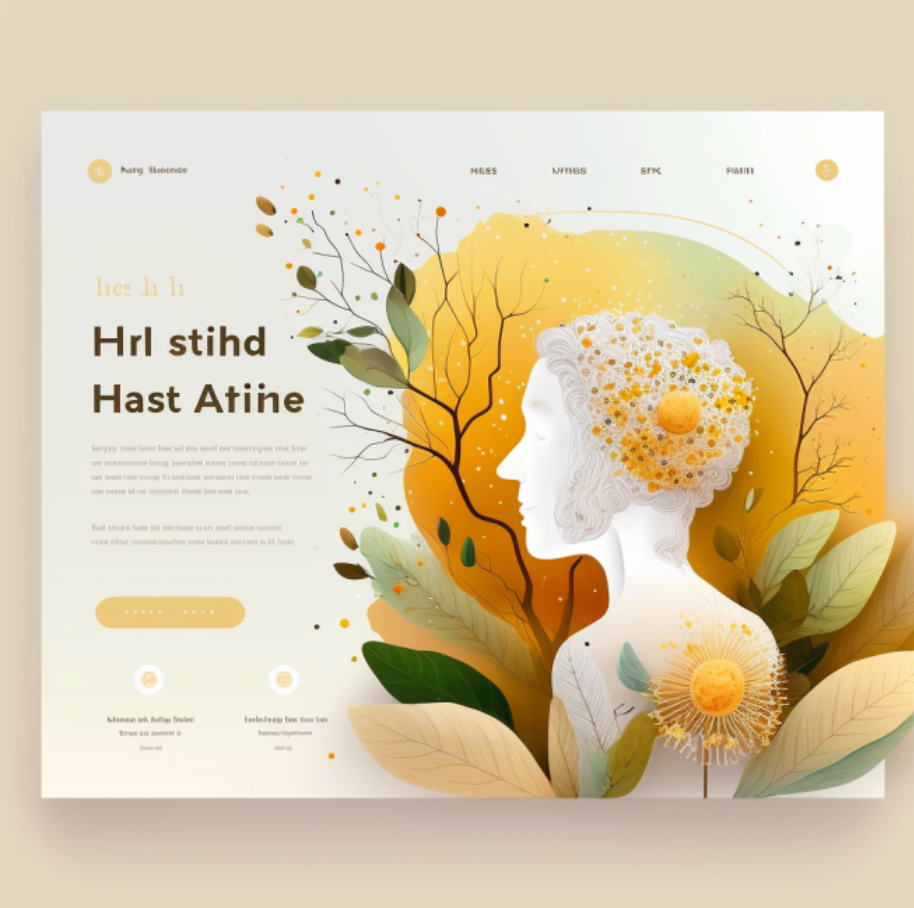
\includegraphics[width = 4in]{frontendwebdev_ex}
    \captionof{figure}{Voorbeeld: Landingspagina op basis van een prompt in Midjourney.}
    \label{fig:frontendwebdev_ex}
\end{center}


\section{Webscraping}
Webscraping is een krachtige techniek die gebruikt kan worden om tekstuele input te verzamelen voor het genereren van kunstwerken. Met webscraping kunnen gegevens van websites worden geëxtraheerd en gebruikt worden als input voor generatieve AI-algoritmen om kunstwerken te genereren. \\
 
Een belangrijke overweging bij het gebruik van webscraping voor het genereren van kunstwerken is het respecteren van de regels en beperkingen van de websites die worden gescraped. Websites kunnen bijvoorbeeld beperkingen opleggen via het robots.txt-bestand, dat aangeeft welke delen van de website geopend kunnen worden voor scraping. Het is belangrijk om deze regels te respecteren en alleen gegevens te verzamelen waarvoor toestemming is verleend. \\

Belangrijke zaken waarmee er rekening gehouden moet worden om een scraper te creeëren volgens \autocite{BIO2014}:

\begin{itemize}
    \item \textbf{Toegang krijgen tot de site:} De webscraper maakt verbinding met de doelwebsite via het HTTP-protocol en houdt rekening met verzoeksmethoden zoals GET en POST. Daarnaast moet de 'User-Agent' correct worden ingesteld.
    \item \textbf{HTML-Parsen en de inhoud extraheren:} De scraper moet in staat zijn om de HTML-structuur van de webpagina te begrijpen en de relevante gegevens te extraheren. Dit kan worden bereikt met behulp van reguliere expressies, HTML-parsing bibliotheken of op selectors gebaseerde talen zoals XPath en CSS-selector syntax.
    \item \textbf{Output:} De geëxtraheerde gegevens moeten worden omgezet in een gestructureerde weergave die geschikt is voor verdere analyse en opslag, zoals in-memory datastructuren of tekstgebaseerde bestandsformaten zoals XML of CSV.
\end{itemize}

\subsection{Ethische aspecten}
\label{subsection:scraper-ethische-aspecten}
Bij het uitvoeren van webscraping-activiteiten is het van belang om ethische overwegingen in acht te nemen. Webscraping kan verschillende ethische uitdagingen met zich meebrengen, zoals het respecteren van de privacy van gebruikers en het naleven van de regels en beperkingen van websites. Hier zijn enkele belangrijke ethische aspecten volgens \autocite{scrape_ethics} om rekening mee te houden tijdens het ontwikkelen van de scraper: 

\begin{itemize}
    \item \textbf{Privacy en persoonlijke gegevens:} Het is essentieel om geen persoonlijke identificeerbare informatie of gevoelige gegevens te verzamelen zonder de toestemming van de gebruikers of de website-eigenaren.
    \item \textbf{Auteursrecht en intellectuele eigendom:} Het is belangrijk om de regels en beperkingen van websites te respecteren met betrekking tot het gebruik en de reproductie van hun inhoud.
    \item \textbf{Serverbelasting:} Webscraping kan de serverbelasting van websites verhogen, vooral als grote hoeveelheden gegevens worden opgevraagd of als frequent en intensief scraping plaatsvindt. Dit kunnen we vermijden door een wachttijd te simuleren na elke request. 
\end{itemize}

\subsection{BeautifulSoup4}
BeautifulSoup4 (BS4) is een populaire Python-bibliotheek voor webscraping die het eenvoudig maakt om gegevens van webpagina's te verkrijgen en te verwerken \autocite{BIO2014, BSFOR2015}. \\

Het biedt een intuïtieve en eenvoudige manier om HTML- en XML-documenten te parseren en gegevens eruit te extraheren. Met BeautifulSoup4 kunnen ontwikkelaars elementen selecteren op basis van tags, klassen, ids en andere attributen. Ze kunnen ook door de hiërarchie van de HTML-structuur navigeren en de gewenste gegevens extraheren. \\

De officiële documentatie van BeautifulSoup4 is een waardevolle bron van informatie en richtlijnen voor het gebruik van de bibliotheek. Het bevat gedetailleerde uitleg, voorbeelden en referenties naar de verschillende functies en methoden van BeautifulSoup4. 
De documentatie is beschikbaar op de volgende website: \autocite{BS4Documentation}. \\


\section{De uitdagingen en beperkingen van AI-gegenereerde kunst}
AI-gegenereerde kunst brengt verschillende uitdagingen en beperkingen met zich mee, die invloed hebben op de creativiteit, originaliteit en interpretatie van de gegenereerde kunstwerken en dus ook het onderzoek zelf.

\subsection{Creativiteit}
Een van de belangrijkste uitdagingen bij AI-gegenereerde kunst is het stimuleren van creativiteit. Hoewel AI in staat is om grote hoeveelheden gegevens te analyseren en patronen te herkennen, mist het vaak de menselijke verbeeldingskracht en intuïtie die nodig zijn voor het creëren van originele en innovatieve kunstwerken. AI-algoritmen zijn gebaseerd op bestaande gegevens en modellen, waardoor ze vaak geneigd zijn om bestaande stijlen en trends te repliceren in plaats van iets volledig nieuws te creëren. Het uitdagen van AI om buiten de gebaande paden te denken en echt unieke kunstwerken te genereren, blijft een grote uitdaging.

\subsection{Originaliteit}
Een andere beperking van AI-gegenereerde kunst is de kwestie van originaliteit. Omdat AI-systemen zijn getraind op bestaande datasets, bestaat het risico dat ze onbedoeld bestaande kunstwerken of ideeën reproduceren zonder voldoende originaliteit toe te voegen. Dit kan leiden tot het genereren van kunstwerken die sterk lijken op bestaande werken of het schenden van auteursrechten. Het waarborgen van voldoende originaliteit in AI-gegenereerde kunst vereist een zorgvuldige afweging tussen het gebruik van bestaande gegevens voor training en het aanmoedigen van nieuwe, unieke expressie.

\subsection{Interpretatie}
Een uitdaging bij het omgaan met AI-gegenereerde kunst is de interpretatie ervan. Omdat kunstwerken vaak worden geassocieerd met emotie, betekenis en subjectiviteit, kan de interpretatie van AI-gegenereerde kunstwerken een uitdaging zijn. Het ontbreekt AI vaak aan de menselijke context en begrip om diepere betekenissen en nuances in kunstwerken te begrijpen. Dit kan resulteren in kunstwerken die voor mensen moeilijk te interpreteren zijn of die niet de gewenste emotionele impact hebben. Het betrekken van menselijke interactie en interpretatie bij AI-gegenereerde kunst kan helpen om deze uitdaging aan te pakken en een meer gelaagde en betekenisvolle ervaring te creëren.

Het is belangrijk om deze uitdagingen en beperkingen in gedachten te houden bij het ontwikkelen en evalueren van AI-gegenereerde kunst. Door voortdurend te streven naar creativiteit, originaliteit en begrijpelijke interpretatie, kunnen we de potentie van AI benutten om nieuwe vormen van artistieke expressie te verkennen en te ontwikkelen.
